\documentclass[letterpaper,11pt]{article}

% Preamble
\usepackage[utf8]{inputenc}
\usepackage{amsmath, amssymb}
\usepackage{graphicx}
\usepackage{hyperref}
\usepackage{geometry}
\usepackage[style=chem-acs]{biblatex}
\addbibresource{references.bib}
\geometry{letterpaper, margin=1in}

\usepackage{setspace}
\doublespacing

\usepackage{lipsum}
\usepackage{multicol}


% Title and author information
\title{Delayed recycle Axial Reactor xxx}
\author{
  Behrad Moadeli\thanks{Ualberta, Address. Email: moadeli@ualberta.ca} \and
  Author Two\thanks{Affiliation, Address. Email: author2@example.com}
}

\date{\today}

\begin{document}

\maketitle

\begin{abstract}
    % Your abstract here
    This is a brief summary of the paper, usually around 150-250 words. \lipsum[1-1]
\end{abstract}
% \begin{multicols}{2}

  \section{INTRODUCTION}

Many chemical, petrochemical, and biochemical unit operation processes are modelled as distributed parameter systems (DPS). When these processes are described using first-principle modeling, they result in a class of partial differential equations (PDEs) to effectively capture diffusion, transport, and reaction phenomena, leading to infinite-dimensional state space representations \autocite{ray1981advanced}. This characteristic presents significant challenges, making the control and estimation of DPS inherently more complex than finite-dimensional systems. Two primary methods have emerged for addressing DPS control. One is early lumping, which approximates the infinite-dimensional system with a finite-dimensional model \autocite{davison1976robust, francis1977linear}. While this method enables the use of standard regulator design techniques, mismatches between the dynamical properties of the original DPS and the approximate lumped parameter model can occur, negatively affecting the performance of the designed regulator \autocite{moghadam2012infinite}. The second method is late lumping, which directly tackles the infinite-dimensional system before applying numerical solutions. This approach introduces a challenging yet fertile direction of research, leading to many meaningful contributions that address various aspects of control and estimation of infinite-dimensional systems.

Among notable studies utilizing late lumping method for control of convection-reaction chemical systems resulting in first order hyperbolic PDEs, \Citeauthor{christofides1998robust} explored the robust control of quasi-linear first-order hyperbolic PDEs, providing explicit controller synthesis formulas for uncertainty decoupling and attenuation \autocite{christofides1998robust}. \Citeauthor{krstic2008backstepping} extended boundary feedback stabilization techniques for first-order hyperbolic PDEs using a backstepping method, converting the unstable PDE into a system for finite-time convergence \autocite{krstic2008backstepping}. Relevant applications of reaction-convection systems other than tubular reactors have also been addressed within this field, resulting in regulator/observer design strategies for chemical systems governed by first order hyperbolic PDEs. \Citeauthor{xu2016state} addressed the state feedback regulator problem for a countercurrent heat exchanger system, utilizing an infinite-dimensional approach to ensure that the controlled output tracks a reference signal \autocite{xu2016state}. Xie and Dubljevic \Citeauthor{xie2021discrete} developed a discrete-time output regulator for gas pipeline networks, emphasizing the transformation of continuous-time models into discrete-time systems while preserving essential continuous-time properties \autocite{xie2021discrete}. This work was further extended by \Citeauthor{zhang2023tracking}, who proposed a tracking model predictive control and moving horizon estimation design for pipeline systems, addressing the challenges of state and parameter estimation in an infinite-dimensional chemical system governed by first order hyperbolic PDEs \autocite{zhang2023tracking}. For a similar convection-reaction system, \Citeauthor{zhang2022dynamic} proposed a model predictive control strategy, incorporating a Luenberger observer to achieve output constrained regulation in a system modeled by nonlinear coupled hyperbolic PDEs \autocite{zhang2022dynamic}. 

Additionally, diffusion-convection-reaction systems resulting in parabolic PDEs are also addressed in several works. For example, \Citeauthor{Christofides2012book} addressed order reduction methods for diffusion-convection-reaction type of reactors \autocite{Christofides2012book}. \Citeauthor{dubljevic2006predictive2} utilized modal decomposition to capture dominant modes of a DPS to construct a reduced order finite dimensional system, which enables the design of a low dimensional controller for a diffusion-convection-reaction type reactor described by second order parabolic PDEs \autocite{dubljevic2006predictive2}. \Citeauthor{ozorio2019heat} designed and compared the performance of a full-state and output feedback controller for a diffusion-convection heat exchanger system \autocite{ozorio2019heat}. In \Citeauthor{khatibi2021model}'s work, an axial dispersion tubular reactor equipped with recycle stream is considered as a second order parabolic DPS, with a predictive controller being utilized to optimally control the reactor \autocite{khatibi2021model}.  Although the presence of recycle is common in industrial reactor designs, this work is one of the few contributions in this field that addresses a diffusion-convection-reaction system equipped with a recycle stream.

Moreover, continuous-time optimal control design is a well-developed concept for distributed parameter systems, particularly when the system generator is either a self-adjoint operator or can be transformed into one through a proper linear transformation \autocite{morrisbook}. However, there are distributed parameter systems that do not possess this property. Instead, the system generator belongs to the domain of Riesz-spectral operators. Rather than an orthonormal basis for the function-space, these generators introduce a bi-orthonormal set of eigenfunctions as the basis. Optimal controller design for these systems was initially addressed in \Citeauthor{curtainbook} \autocite{curtainbook}. Since then, significant work has been done in this field. For instance, continuous-time optimal control design for a cracking catalytic reactor, another convection-reaction system governed by first-order hyperbolic PDEs, has been achieved by solving an operator Riccati equation (ORE)\autocite{aksikas2009lq}. This work has been further extended to time-varying PDEs of the same class\autocite{aksikas2013optimal}. The same approach has been applied to develop a full-state feedback\autocite{mohammadi2012lq} and output feedback\autocite{aksikas2024spectral} linear quadratic (LQ) optimal regulator for a boundary-controlled convection-reaction system, utilizing the properties of a Riesz-spectral generator for the system.

On top of those dynamic systems that are distributed in space, delay systems are another example of distributed parameter systems \autocite{curtainbook}. Although delay is commonly represented in the form of delay differential equations (DDEs), it can also be modeled as a transport partial differential equation (PDE), which offers advantages in more complex scenarios or when employing alternative norms on infinite-dimensional states. This approach allows for a smoother transition to problems involving more intricate PDE dynamics while maintaining notational consistency \autocite{krstic2009book}. Input/output delay with relevant applications in chemical engineering has been addressed previously in the field of control theory for DPS. For example, time-delayed boundary observation is considered while addressing an output feedback regulator for a tubular reactor \autocite{Guilherme2019ACC}. However, the notion of state-delay (as opposed to delayed-input or delayed-output) seems to be less addressed in this field compared to other relevant fields like signal processing, self-driving cars, or network control theory (NCT). This is probably because not much application in the field of distributed parameter chemical engineering systems can be introduced in the first place. \Citeauthor{ozorio2019heat}'s work is one of the few instances that addressed a delayed-state distributed parameter chemical engineering system \autocite{ozorio2019heat}, where they designed a full-state and output feedback regulator for a system of heat exchangers. The notion of state-delay comes from the time it takes for a stream to leave one pass of the heat exchanger and enter the next pass. As stated previously, not much work is published addressing chemical reactors equipped with recycle as distributed parameter systems. Even in \Citeauthor{khatibi2021model}'s work, the recycle is assumed to be instantaneous; a simplifying assumption that does not resonate well with reality. In fact, taking the time it takes for the recycle stream to re-enter the reactor input can be another instance for the rare concept of a delayed state DPS in the field of chemical engineering. In another attempt, \Citeauthor{qi2021output} addressed the challenge of state delay imposed by a recycle stream in a system modeled by interconnected first-order hyperbolic PIDEs, introducing a transport PDE to account for the in-domain recycle delay \autocite{qi2021output}. However, the diffusion term was not addressed, leaving a gap in the literature regarding diffusion-convection-reaction systems with a recycle stream imposing state delay.

The present work focuses on the control of an axial tubular reactor equipped with a recycle stream, a configuration common in industrial processes but inadequately addressed in the literature. Unlike previous studies that assumed instantaneous recycle, this work incorporates the time delay associated with the recycle stream re-entering the reactor, presenting a rare example of state-delay in the field of chemical engineering DPS. The model comprises a second-order parabolic PDE to capture the diffusion-convection-reaction nature of the reactor, coupled with a first-order hyperbolic PDE to account for the delay. The boundary conditions are chosen as Danckwerts boundary conditions, which are particularly suitable for this type of reactor. The system results in a non-self-adjoint operator, but by utilizing the bi-orthogonal theorem, given that the generator is Riesz-spectral, a full-state feedback optimal LQ regulator is developed, followed by an output feedback regulator. The control strategy is derived by solving an operator Riccati equation (ORE) and employs a late lumping approach. Actuation and observation are conducted at the boundaries, making it a boundary-actuated system involving finite-dimensional dynamics for an infinite-dimensional DPS. The paper is structured as follows:

\begin{itemize}
    \item System analysis: Modeled the delay infinite-dimensional system (DPS) and transformed it into a system of coupled PDEs using the delay-transport approach. Explored the characteristics of the system by examining eigenvalues, the adjoint operator, followed by introducing the bi-orthogonal basis
    \item Full-state feedback regulator: Developed the design strategy for optimal full-state regulator by formulating the infinite-time horizon LQ control problem, converting the ORE into matrix Riccati equations (MRE), and calculating the feedback gain.
    \item Output feedback compensator: Addressed practical limitations of the proposed full-state feedback mechanism by introducing a Luenberger observer for state reconstruction, followed by the design of an output feedback regulator.
    \item Numerical simulation: Provided an illustrative numerical example to demonstrate the practical application of the theoretical concepts developed; i.e. the open-loop response, in addition to the closed-loop system equipped with both full-state feedback regulator and output feedback compensator.
\end{itemize}
  
  \section{Open-loop System}

\subsection{System Model}

The chemical process illustrated in Figure~\ref{fig:reactor_scheme} represents an axial dispersion tubular reactor, which incorporates diffusion, convection, and a first-order irreversible chemical reaction \autocite{levenspiel1998chemical}. The reactor is equipped with a recycle mechanism, allowing a fraction of the product stream to re-enter the reactor to ensure the consumption of any unreacted substrate. By applying first-principle modeling through relevant mass balance relations on an infinitesimally small section of the reactor, the reactor's dynamics can be described by a second-order parabolic PDE, a common class of equations used to characterize diffusion-convection-reaction systems \autocite{jensen1982bifurcation}. The resulting PDE that describes the reactor model is given by:

\begin{equation} \label{eq:PDE_original_model}
    \dot{x}(\zeta, t) = D \partial_{\zeta \zeta} c(\zeta, t) - v \partial_\zeta c(\zeta, t) + k_r c(\zeta, t)
\end{equation}

subject to Dankwerts boundary conditions:

\begin{align} \label{eq:BC}
    \begin{cases}
        &D \partial_\zeta c(0, t) - v c(0, t) = -v \left[ R c(1, t-\tau) + (1-R) u(t) \right] \\
        &\partial_\zeta c(1, t) = 0 \\
        &y(t) = c(1, t)
    \end{cases}
\end{align}

Here, $c(\zeta, t)$ denotes the properly scaled notion of concentration along the reactor, representing the state of the system. The physical parameters $D$, $v$, $k_r$, $R$, and $\tau$ correspond to the diffusion coefficient, flow velocity along the reactor, reaction constant, recycle ratio, and residence time of the recycle stream, respectively. The spatial and temporal coordinates of the system are represented by $\zeta$ and $t$, where $\zeta \in [0, 1]$ and $t \in [0, \infty)$.

Dankwerts boundary conditions are particularly suitable for modeling axial tubular reactors, as they account for deviations from perfect mixing and piston flow, assuming negligible transport lags in connecting lines \autocite{danckwerts1993continuous}. These conditions make the model more realistic for chemical reactors of this type. The input and the output of the system are also present in the boundary conditions. The system output is measured at the reactor outlet, while the input is applied at the inlet. Additionally, the delayed state resulting from the recycled portion of the flow, occurring $\tau$ time units ago, is incorporated into the inlet; all as shown in Equation~\ref{eq:BC}.


\begin{figure}[ht]
    \centering
    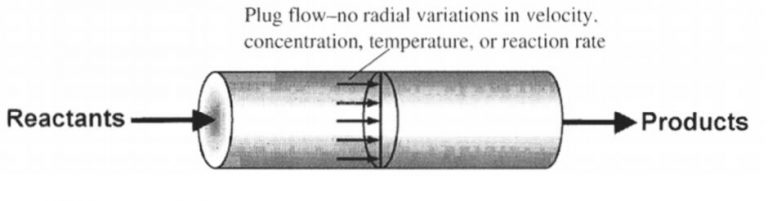
\includegraphics[width=0.7\textwidth]{Figures/sample.jpeg}
    \caption{Sample figure.}
    \label{fig:reactor_scheme}
\end{figure}

\subsection{PDE Representation of Delay Term}

One effective method for addressing delay in systems is to represent the delay using an alternative transport partial differential equation (PDE). This approach is particularly advantageous when the problem already involves similar forms of PDEs, as is the case in the current study. To specifically address the delay in the system under consideration, the state variable $c(\zeta, t)$ is expanded into a vector of functions $x(\zeta, t) \equiv [x_1(\zeta, t), x_2(\zeta, t)]^T$, where $x_1(\zeta, t)$ represents the concentration within the reactor, and $x_2(\zeta, t)$ is introduced as a new state variable to account for the concentration along the recycle stream. The delay is thus modeled as a pure transport process, wherein the first state $x_1(\zeta, t)$ is transported from the reactor outlet to the inlet, experiencing a delay of $\tau$ time units while in the recycle stream. As a result, Equations~\ref{eq:PDE_original_model}~and~\ref{eq:BC} may be re-formulated as follows:

\begin{align}
    \partial_t 
    \begin{bmatrix}
        x_1(\zeta, t) \\ x_2(\zeta,t)
    \end{bmatrix}
    =
    \begin{bmatrix}
        D \partial_{\zeta \zeta} - v \partial_\zeta + k_r && 0 \\
        0 && -\frac{1}{\tau} \partial_\zeta
    \end{bmatrix}
    \begin{bmatrix}
        x_1(\zeta, t) \\ x_2(\zeta,t)
    \end{bmatrix}\\
\begin{cases}
    D \partial_\zeta x_1(0, t) - v x_1(0, t) = -v \left[ R x_2(0, t) + (1-R) u(t) \right] \\
    \partial_\zeta x_1(1, t) = 0 \\
    x_1(1,t) = x_2(1,t) \\
    y(t) = x_1(1, t)
\end{cases}
\end{align}

With all state variables now expressed explicitly at a specific time instance $t$—in contrast to the previous representation where states at $t$ were directly involved with states at $(t-\tau)$—the system can be described in the standard state-space form of an infinite-dimensional linear time-invariant (LTI) system as $\dot{x} = \mathfrak{A} x$. Here, the state $x(\zeta, t) = [x_1(\zeta, t), x_2(\zeta, t)]^T$ is a vector of functions, and $\mathfrak{A}$ is a linear operator $\mathcal{L}(X)$ acting on a Hilbert space $X: L^2[0,1] \times L^2[0,1]$. The operator $\mathfrak{A}$ and its domain are defined in detail as shown in Equation~\ref{eq:operator_A}:

\begin{equation} \label{eq:operator_A}
    \begin{aligned}
        \mathfrak{A} \equiv&
        \begin{bmatrix}
            D \partial_{\zeta \zeta} - v \partial_\zeta + k_r & 0 \\
            0 & \frac{1}{\tau} \partial_\zeta
        \end{bmatrix}\\
        D(\mathfrak{A}) =& \Bigl\{ x = [x_1, x_2]^T \in X:
        x(\zeta), \partial_\zeta x(\zeta), \partial_{\zeta \zeta} x(\zeta) \quad \mathrm{a.c.},\\
        &D \partial_\zeta x_1(0) - v x_1(0) = -v \left[ R x_2(0) + (1-R) u \right],\\
        &\partial_\zeta x_1(1) = 0,
        x_1(1) = x_2(1) \Bigr\}
    \end{aligned}
\end{equation}

\subsection{Adjoint Operator}

The adjoint operator $\mathfrak{A}^*$ plays a critical role in analyzing the spectral properties of the system. It is obtained in Equation~\ref{eq:adjoint_A}:

\begin{equation} \label{eq:adjoint_A}
    \begin{aligned}
        \langle \mathfrak{A} \phi, \psi\rangle  = \langle \phi, {\mathfrak{A}}^{*} \psi\rangle  &\Rightarrow \\
        {\mathfrak{A}}^{*} =&
        \begin{bmatrix}
            D \partial_{\zeta \zeta} + v \partial_\zeta +k_r & 0\\
            0 & -\frac{1}{\tau} \partial_\zeta
        \end{bmatrix}\\
        D(\mathfrak{A}^*) =& \Bigl\{ y = [y_1, y_2]^T \in Y:
        y(\zeta), \partial_\zeta y(\zeta), \partial_{\zeta \zeta} y(\zeta) \quad \mathrm{a.c.},\\
        &D \partial_\zeta y_1(1) + v y_1(1) = \frac{1}{\tau} y_2(1) \\
        &R v y_1(0) = \frac{1}{\tau} y_2(0) \\
        &\partial_\zeta y_1(0) = 0 \Bigr\}
    \end{aligned}
\end{equation}

where $\phi_i(\zeta) = [\phi_{i,1}(\zeta), \phi_{i,2}(\zeta)]^T$ and $\psi_i(\zeta) = [\psi_{i,1}(\zeta), \psi_{i,2}(\zeta)]^T$ are the eigenfunction of $\mathfrak{A}$ and $\mathfrak{A}^*$, respectively. Given that $\mathfrak{A}$ is not self-adjoint (i.e., $\mathfrak{A} \neq \mathfrak{A}^*$), their combined eigenmodes may still form a bi-orthonormal basis, typical of a Riesz-spectral operator \autocite{curtainbook}. Therefore their spectral properties must be determined by solving their characteristic equations.

\subsection{Eigenvalue Problem}

The eigenvalue problem\autocite{pdebook} for $\mathfrak{A}$ is formulated as:

\begin{equation} \label{eq:eig_prob}
        \mathfrak{A} \phi_i(\zeta) = \lambda_i \phi_i(\zeta)
\end{equation}

% \begin{equation} \label{eq:eigval_calc_1}
%     \begin{aligned}
%         &\begin{cases}
%             &\lambda \phi_1 = D \frac{d^2 \phi_1}{d \zeta ^2}  - v \frac{d \phi_1}{d \zeta} + k \phi_1 \\
%             &\lambda \phi_2 = \frac{1}{\tau} \frac{d \phi_2}{d \zeta}
%         \end{cases} \\ B.C. &\begin{cases}
%             &D \left. \frac{d \phi_1}{d \zeta} \right|_{\zeta=0} - v \left. \phi_1 \right|_{\zeta=0} = - R v \left. \phi_2 \right|_{\zeta=0} \\
%             &\left. \phi_1 \right|_{\zeta=1} = 0 \\
%             &\left. \phi_1 \right|_{\zeta=1} = \left. \phi_2 \right|_{\zeta=1}
%         \end{cases}
%     \end{aligned}
% \end{equation}

where $\lambda_i \in \mathbb{C}$ is the $i^{\text{th}}$ eigenvalue. To obtain the characteristic equation, the system of PDEs shall be reduced to the ODE system in Equation~\ref{eq:eigval_calc_2} $\forall i \geq 0$:

\begin{equation} \label{eq:eigval_calc_2}
    \begin{aligned}
        \partial_\zeta \begin{bmatrix}
            \phi_1 \\ \partial_\zeta \phi_1 \\ \phi_2
        \end{bmatrix} = \begin{bmatrix}
            0 & 1 & 0 \\
            \frac{\lambda-k_r}{D} & \frac{v}{D} & 0 \\
            0 & 0 & \tau \lambda 
        \end{bmatrix} \begin{bmatrix}
            \phi_1 \\ \partial_\zeta \phi_1 \\ \phi_2
        \end{bmatrix}
    \end{aligned}
\end{equation}

which is in the form of $ \tilde{\phi}_\zeta  = \tilde{\mathfrak{A}} \tilde{\phi}$, with the solution stated in Equation~\ref{eq:eigval_calc_3}:

\begin{equation} \label{eq:eigval_calc_3}
    \begin{bmatrix}
        \phi_1 \\ \partial_\zeta \phi_1 \\ \phi_2
    \end{bmatrix}_{\zeta=1} = \begin{bmatrix}
        \Lambda_{1,1} & \Lambda_{1,2} & \Lambda_{1,3} \\
        \Lambda_{2,1} & \Lambda_{2,2} & \Lambda_{2,3} \\
        \Lambda_{3,1} & \Lambda_{3,2} & \Lambda_{3,3}
    \end{bmatrix} \begin{bmatrix}
        \phi_1 \\ \partial_\zeta \phi_1 \\ \phi_2
    \end{bmatrix}_{\zeta=0}
\end{equation}

where the matrix $\Lambda_{(i,j)}$ is defined as $e^{\tilde{\mathfrak{A}}}$. By applying the boundary conditions to Equation~\ref{eq:eigval_calc_3}, the algebraic system of equations in Equation~\ref{eq:eigval_calc_4} is obtained:

\begin{equation} \label{eq:eigval_calc_4}
    \begin{bmatrix}
        -v & D & Rv \\
        \Lambda_{2,1} & \Lambda_{2,2} & \Lambda_{2,3} \\
        (\Lambda_{1,1} - \Lambda_{3,1}) & (\Lambda_{1,2} - \Lambda_{3,2}) & (\Lambda_{1,3} - \Lambda_{3,3})
    \end{bmatrix} \begin{bmatrix}
        \phi_1 \\ \partial_\zeta \phi_1 \\ \phi_2
    \end{bmatrix}_{\zeta=0} = \tilde{\Lambda} \tilde{\phi}_{\zeta = 0} = 0
\end{equation}

where $\tilde{\Lambda}$ is defined as the square matrix shown in Equation~\ref{eq:eigval_calc_4}. Equation~\ref{eq:eigval_calc_4} suggests that the matrix $\tilde{\Lambda}$ must be rank-deficient for appropriate values of $\lambda_i$. Attempts to analytically solve the characteristic equation $det(\tilde{\Lambda}) = 0$ has failed; therefore, it is solved numerically using the parameters in Table~\ref{tab:pars}. The resulting eigenvalue distribution is depicted in Figure~\ref{fig:eigval_dist} in the complex plane.

\begin{table}[ht]
    \centering
    \caption{Physical Parameters for the System}
    \label{tab:pars}
    \begin{tabular}{|c|c|c|c|}
    \hline
    \textbf{Parameter}        & \textbf{Symbol} & \textbf{Value}     & \textbf{Unit}    \\ \hline
    Diffusivity               & $D$             & $2\times10^{-5}$   & ${m^2}/{s}$      \\ \hline
    Velocity                  & $v$             & $1\times10^{-2}$   & ${m}/{s}$        \\ \hline
    Reaction Constant         & $k_r$           & $1.5$              & $s^{-1}$         \\ \hline
    Recycle Residence Time    & $\tau$          & $80$               & $s$              \\ \hline
    Recycle Ratio             & $R$             & $0.3$              & $-$              \\ \hline
    \end{tabular}
\end{table}

\begin{figure}[ht]
    \centering
    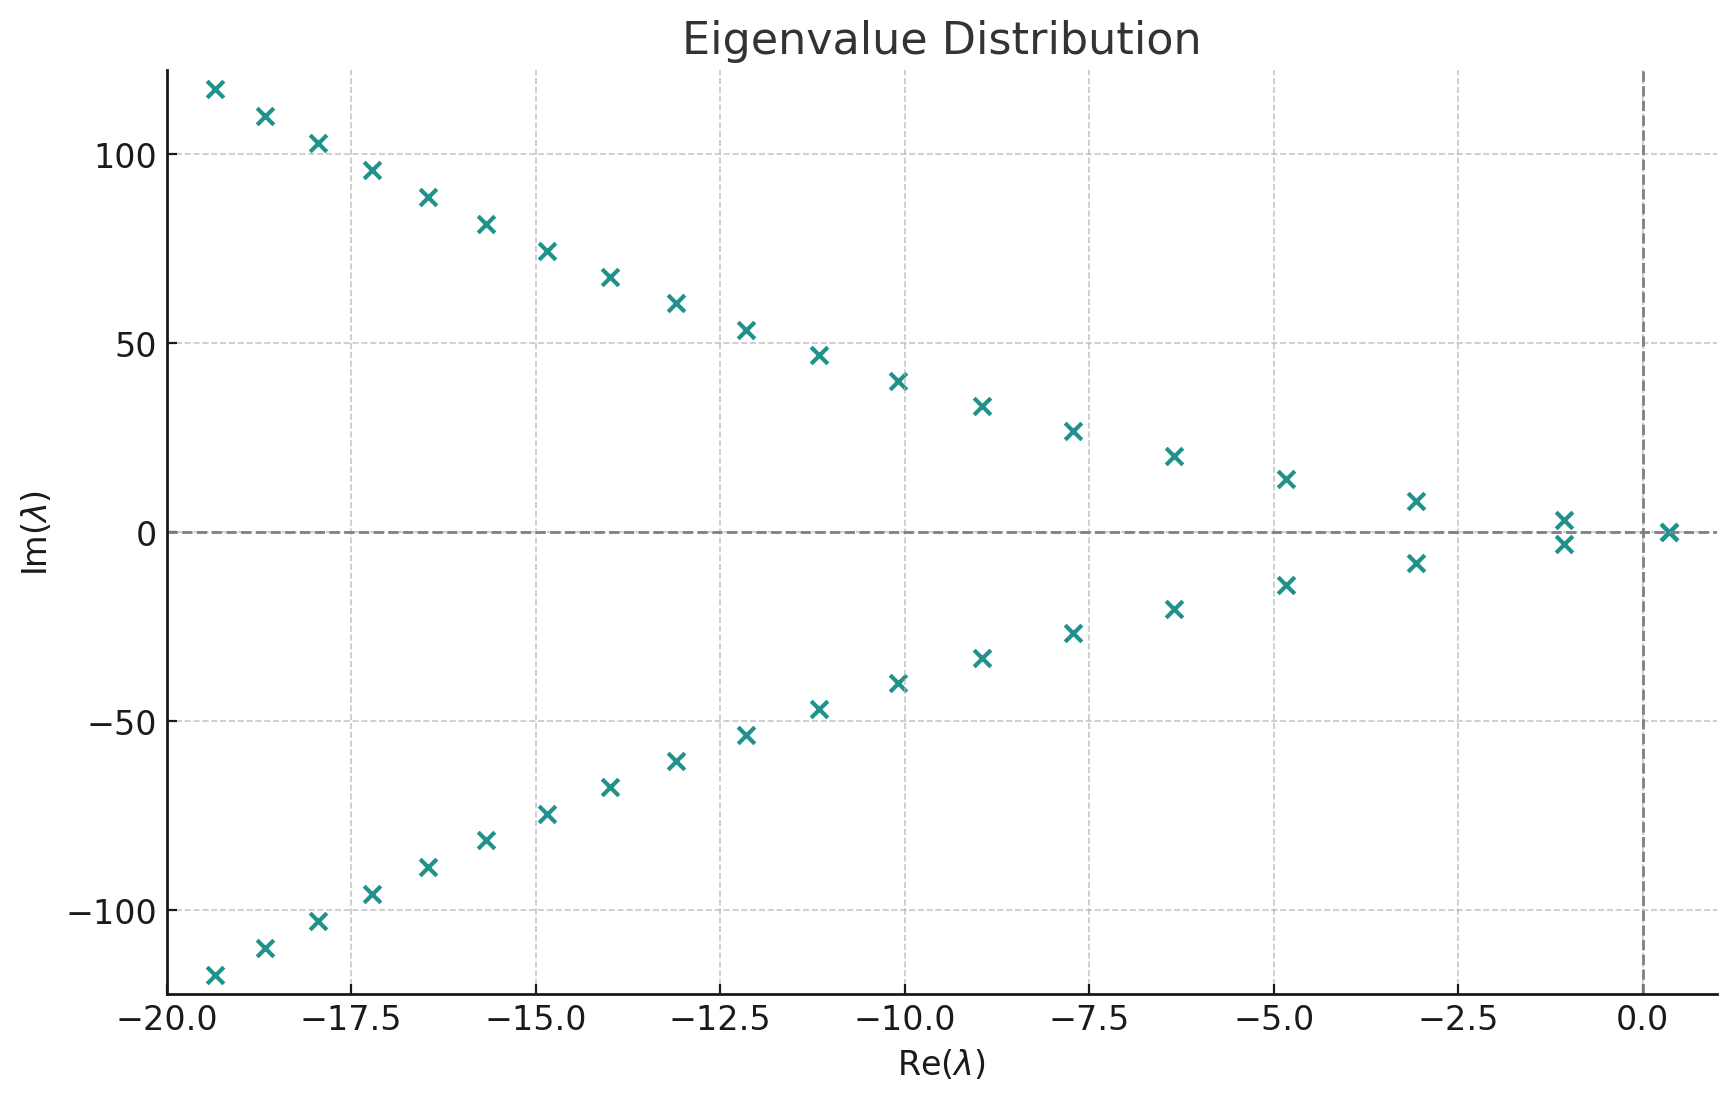
\includegraphics[width=0.7\textwidth]{Figures/eigval_dist_R_0.3.jpg}
    \caption{Eigenvalues of operator $\mathfrak{A}$ plotted on complex plane}
    \label{fig:eigval_dist}
\end{figure}

Following the same procedure for $\mathfrak{A}^*$ shows that the eigenvalues of $\mathfrak{A}$ match the ones of its adjoint, confirming that $\mathfrak{A}$ and $\mathfrak{A}^*$ form a bi-orthogonal basis according to Equation~\ref{eq:biorth}:

\begin{equation} \label{eq:biorth}
    \begin{aligned}
        &\langle \mathfrak{A} \phi_i, \psi_j \rangle = \langle \lambda_i \phi_i, \psi_j \rangle = \lambda_i \langle \phi_i, \psi_j \rangle \\
        \text{L.H.S.} = &\langle \phi_i, \mathfrak{A}^* \psi_j \rangle = \langle \phi_i, \lambda_j^* \psi_j \rangle = \overline{\lambda_j^*} \langle \phi_i, \psi_j \rangle \\
        &\lambda_i = \overline{\lambda_i^*} \Rightarrow \langle \phi_i, \psi_j \rangle = \delta_{ij}
    \end{aligned}
\end{equation}

The eigenfunctions $\{ \phi_i(\zeta), \psi_i(\zeta) \}$ (for $\mathfrak{A}$ and $\mathfrak{A}^*$, respectively) may be obtained following the calculation of eigenvalues. The first 3 eigenfunctions are plotted in Figure~\ref{fig:eigfun}. 

\begin{figure}[ht]
    \centering
    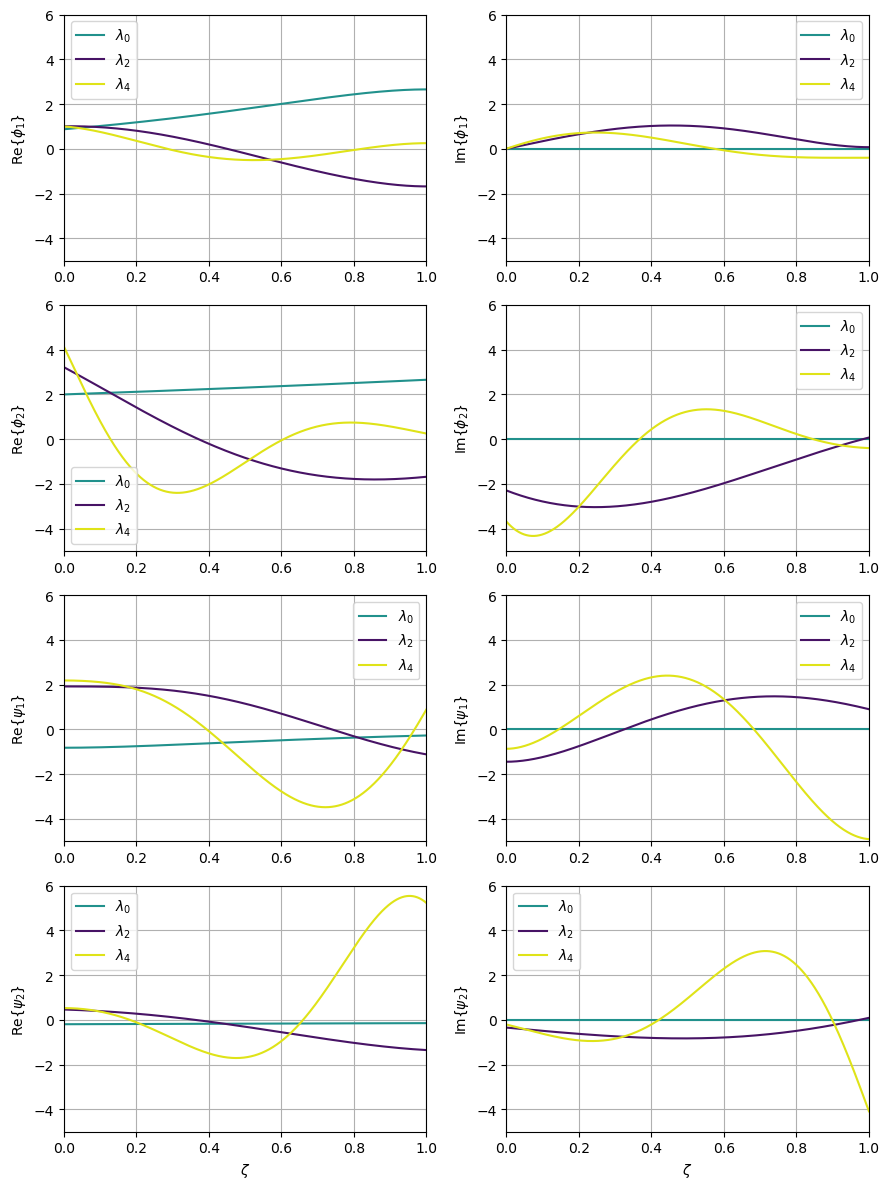
\includegraphics[width=0.7\textwidth]{Figures/eigfuns.png}
    \caption{First few eigenmodes of $\mathfrak{A}$ and $\mathfrak{A}^*$}
    \label{fig:eigfun}
\end{figure}

  
  \section{Full-state Feedback Regulator}

Having the Riesz-spectral operator $\mathfrak{A}$ generate a bi-orthogonal basis provides the foundation for solving the Operator Riccati Equation (ORE) in this chapter, a crucial step in Linear Quadratic Regulator (LQR) design. The aim of solving the ORE is to find a feedback control law that minimizes an infinite-time cost function given in Equation~\ref{eq:cost_fun}:

\begin{equation} \label{eq:cost_fun}
    J(x_0, u) \int_0^{\infty} \langle x(s), \mathfrak{Q} x(s)\rangle + \langle u(s), \mathfrak{R} u(s)\rangle ds
\end{equation}

where $\mathfrak{Q}$ and $\mathfrak{Q}$ are positive semi-definite matrices of operators of the appropriate size that contribute to the penalty terms due to the costs of state deviation and control action, respectively.

\subsection{Operator Riccati Equation}

The corresponding ORE provides the solution of LQR problem, minimizing the stated cost function. This is done by calculating the positive semi-definite operator $\mathbf{\Pi}$ as the unique solution to the Equation~\ref{eq:ORE_1}, which is later used to obtain the feedback gain, resulting in optimal control of the system.

\begin{equation} \label{eq:ORE_1}
    \langle \mathfrak{A}^* \mathbf{\Pi} x, y\rangle + \langle \mathbf{\Pi} \mathfrak{A} x, y \rangle - \langle \mathbf{\Pi} \mathfrak{B} \mathfrak{R}^{-1} \mathfrak{B}^* \mathbf{\Pi} x, y\rangle + \langle \mathfrak{Q} x, y\rangle = 0
\end{equation}

where $x,y \in D(\mathfrak{A})$. Since the solution to the ORE is unique given any set of functions in the domain of the given operators, one can arbitrarily choose $x = \phi_m$ and $y = \phi_n$, the eigenfunctions of the operator $\mathfrak{A}$ obtained previously. Applying this, in addition to the fact that the operator $\mathbf{\Pi}$ is self-adjoint leads to the following Equation~\ref{eq:ORE_2}:

\begin{equation} \label{eq:ORE_2}
    \langle \mathbf{\Pi} \phi_m, \mathfrak{A} \phi_n \rangle
    + \langle \mathfrak{A} \phi_m, \mathbf{\Pi} \phi_n \rangle
    - \mathfrak{R}^{-1} \langle \mathfrak{B}^* \mathbf{\Pi} \phi_m, \mathfrak{B}^* \mathbf{\Pi} \phi_n\rangle 
    + \langle \mathfrak{Q} \phi_m, \phi_n\rangle = 0
\end{equation}

Knowing that the domain and the range of $\mathbf{\Pi}$ should match the domain of $\mathfrak{A}$ and the domain of $\mathfrak{A}^*$, respectively, operator $\mathbf{\Pi}$ may be represented as the infinite sum given in Equation~\ref{eq:P}:

\begin{equation} \label{eq:P}
    \mathbf{\Pi} x = \sum_{i=1}^{\infty}\sum_{j=1}^{\infty} p_{i,j} \langle x, \psi_j \rangle \psi_i \qquad
    \forall {i,j}: \quad p_{i,j} \in \mathbb{C}
\end{equation}

where $p_{i,j}$ may be seen as scalar elements of an infinite-dimensional square matrix $P$ which can be equivalently used to represent the operator $\mathbf{\Pi}$. This is the first step of converting ORE to its alternative MRE.

\subsection{Obtaining $\mathfrak{B}$ and $\mathfrak{B}^*$}

It is critical to define the operators $\mathfrak{B}$ and $\mathfrak{B}^*$ before proceeding with further simplifying the ORE. Since the system described in the previous section is a boundary-control problem, the operator $\mathfrak{B}$ may be defined according to Equation~\ref{eq:B}:

\begin{equation} \label{eq:B}
    \mathfrak{B} u \equiv
    \begin{bmatrix}
       \delta(\zeta) \\ 0
    \end{bmatrix} \cdot u
\end{equation}

where $\delta(\zeta)$ is the dirac delta function, projecting $u \in \mathbb{R}^1$ to the states function space $X: L^2[0,1] \times L^2[0,1]$. furthermore, operator $\mathfrak{B}^*$ is obtained utilizing adjoint operator properties as shown in Equation~\ref{eq:B*_1}

\begin{equation} \label{eq:B*_1}
    \begin{aligned}
        \langle \mathfrak{A} x + \mathfrak{B} u, y \rangle
        &= \langle \mathfrak{A} x, y \rangle
        + \langle \mathfrak{B} u, y \rangle
        = \langle x, \mathfrak{A}^* y\rangle
        + \langle u, \mathfrak{B}^* y \rangle \\
        \Rightarrow \langle u, \mathfrak{B}^* y \rangle
        &= \langle \mathfrak{A} x + \mathfrak{B} u, y \rangle
        - \langle x, \mathfrak{A}^* y\rangle
    \end{aligned}
\end{equation}

Performing integration by parts resulting from inner products given in Equation~\ref{eq:B*_1} while considering the proper domains for $\mathfrak{A}$ and $\mathfrak{A}^*$ according to Equations~\ref{eq:operator_A}~and~\ref{eq:adjoint_A} results in the expression given in Equation~\ref{eq:B*_2} for $\mathfrak{B}^*$.

\begin{equation} \label{eq:B*_2}
    \mathfrak{B}^* (.) = \Bigl[ v(1-R) \int_0^1 \delta(\zeta) (.) d\zeta \quad , \quad 0 \Bigr]
\end{equation}

\subsection{Matrix Riccati Equation}


  
  \subsection{Output Feedback Compensator}

In the previous work, the optimal regulator was designed under the assumption that it had full access to the system's states, utilizing the inner product of the feedback gain and the states. However, this assumption is not feasible in realistic applications. To address this, an observer is introduced to estimate and reconstruct the states by measuring the system's output in real time. The output, in this context, is taken as the concentration at the reactor outlet, as defined in Equation~\ref{eq:BC}. This leads to the definition of the output operator $\mathfrak{C}$ in the linear time-invariant (LTI) system $\mathbf{\Sigma(\mathfrak{A},\mathfrak{B},\mathfrak{C},-)}$, which is subsequently used to determine the observer gains. The formulation is shown in Equation~\ref{eq:C}:

\begin{equation} \label{eq:C}
    \mathfrak{C} \equiv \begin{bmatrix}
        \int_0^1 \delta(\zeta-1) (.) d\zeta \quad , \quad 0
    \end{bmatrix}
\end{equation}

where $\delta(\zeta)$ denotes the Dirac delta function. Regarding the choice of observer, Luenberger-based observers are well-suited for infinite-dimensional systems when the system parameters are perfectly known \autocite{ali2015reviewobserver}. Among the various methods to compute the gain for this class of observers, pole-placement is a solid, straightforward, and reliable approach for state reconstruction. To ensure that the state reconstruction dynamics converge more quickly than the regulation dynamics, the poles of the observer-based controller are placed to the left of the poles of the full-state feedback controller. This practice is common in the design of observer-based controllers for infinite-dimensional systems \autocite{morrisbook}.

(Sample Diagram)

\begin{tikzpicture}[auto, node distance=2cm,>=latex]
    % Define block styles
    \tikzstyle{block} = [draw, fill=white, rectangle, minimum height=3em, minimum width=3em]
    \tikzstyle{sum} = [draw, fill=white, circle, node distance=1.5cm]
    \tikzstyle{input} = [coordinate]
    \tikzstyle{output} = [coordinate]
    
    % Nodes
    \node [input, name=input] {};
    \node [sum, right of=input] (sum) {};
    \node [block, right of=sum] (B) {$B$};
    \node [block, right of=B] (int) {$\int$};
    \node [block, right of=int] (C) {$C$};
    \node [output, right of=C] (output) {};
    \node [block, below of=B] (A) {$A$};
    \node [block, below of=A] (K) {$-K$};
  
    % Connections
    \draw [draw,->] (input) -- node {$u$} (sum);
    \draw [->] (sum) -- (B);
    \draw [->] (B) -- (int);
    \draw [->] (int) -- (C);
    \draw [->] (C) -- node [name=y] {$y$} (output);
    \draw [->] (int) |- (A);
    \draw [->] (A) -| (sum);
    \draw [->] (A) -- (K);
    \draw [->] (K) -- (sum);
  \end{tikzpicture}

% To implement this, the eigenvalues of the closed-loop system with large real parts were sufficiently shifted to the left of the complex plane, ensuring that the maximum real parts of the observer-based poles satisfy Equation~\ref{eq:obsv_pole}.

% \begin{equation} \label{eq:obsv_pole}
%     \forall i: \quad
%     \mathfrak{Re}(\lambda_i^{\mathrm{obsv}}) \leq 3 \times
%     \max{\Biggl\{
%         \mathfrak{Re}
%             \Bigl(
%                 \sigma\bigl(
%                     \mathfrak{A}-\mathfrak{B}k
%                 \bigr)
%             \Bigr)
%         \Biggr\}}
% \end{equation}

% where $\lambda_i^{\mathrm{obsv}}$ is the $i^{\text{th}}$ eigenvalue of the observer-based regulator, and $\sigma\bigl(\mathfrak{A}-\mathfrak{B}k\bigr)$ refers to the spectrum of the closed-loop system quipped with full-state feedback. This will guarantee the desired faster state reconstruction dynamics compared to regulator stabilization dynamics.

% \begin{itemize}
%     \item Briefly discuss the performance of full-state feedback in control systems.
%     \item Highlight the limitations and challenges associated with full-state feedback.
%     \item Introduce the concepts of state reconstruction and compensator design.
%     \item Present a block diagram illustrating the full-state regulation and compensator approach.
%     \item Define the system output and the output matrix \( C \).
%     \item Explore the criteria for choosing an appropriate observer.
%     \item Describe the method used for calculating the observer gain \( L \) and justify the choice.
%     \item Explain how the observer gain \( L \) is implemented in the control system.
% \end{itemize}

  
  \section{Conclusion}


  \section{Conclusion}

  
  \printbibliography

% \end{multicols}


\end{document}
